\chapter{PmodCLP}

Der PmodCLP besteht aus einem Samsung KS0066 LCD Controller und einem Sunlike LCD Panel, worüber Informationen dargestellt werden können. Es ist möglich 32 Positionen auf dem 16x2 LCD Panel zu nutzen. Pro Position werden die Zeichen dabei mit einer Auflösung von 5x8 angezeigt. \newline

Das System besteht im Wesentlichen aus drei Komponenten. Der character-generator ROM (CGROM) hält 192 vordefinierte Zeichen, darunter 93 ASCII Charaktere. Anschaulich gesehen können die Zeichen über eine matrixartige Struktur indiziert werden, welche im Datenblatt festgelegt ist. Neben den nicht-volatilen Daten im CGROM ist es möglich bis zu 8 eigene Zeichen volatil im character-generator RAM (CGRAM) zu halten. Um nun Zeichen aus diesen beiden Repositories auf dem Panel anzeigen zu können, gibt es den data RAM (DDRAM). Hier können bis zu 80 Zeichencodes gespeichert werden. Er fungiert als Indexspeicher für Daten innerhalb des CGROM oder CGRAM. Wird ein Index aus der matrixartigen Struktur in den DDRAM geladen, erscheint das entsprechende Zeichen auf dem Display. \newline

Das Display selbst verfügt über 2 Zeilen á 16 Positionen. Insgesamt stehen jedoch nicht 32 Speicherplätze zur Verfügung, sondern 39, um beispielsweise Scrolling zu verwenden. \newline

Wichtige Schnittstellen des Samsung KS0066 LCD Controller sind

\begin{itemize}
    \item \textit{DB4-DB7}: Datenbits im Nibble-Mode zur Codierung von Befehlen/Zeichen
    \item \textit{RS (Register Select)}: High für Daten, Low für Instruktionen
    \item \textit{RW (Read/Write)}: High = Read, Low = Write
    \item \textit{E (Enable)}: High für Read, Falling Edge für Write
\end{itemize}

Um diese nutzen zu können wird folgendes Mapping auf dem FPGA hinterlegt:\newline

\begin{lstlisting}[language=bash,caption={Pin-Zuordnung im Constraints-File},breaklines=true,captionpos=b,basicstyle=\footnotesize\ttfamily,
    label={lst:fpga_pins}]
set_property -dict {PACKAGE_PIN D13 IOSTANDARD LVCMOS33}[get_ports{clp_db_tri_io[4]}];#db04
set_property -dict {PACKAGE_PIN B18 IOSTANDARD LVCMOS33}[get_ports{clp_db_tri_io[5]}];#db05
set_property -dict {PACKAGE_PIN A18 IOSTANDARD LVCMOS33}[get_ports{clp_db_tri_io[6]}];#db06
set_property -dict {PACKAGE_PIN K16 IOSTANDARD LVCMOS33}[get_ports{clp_db_tri_io[7]}];#db07
set_property -dict {PACKAGE_PIN E2 IOSTANDARD LVCMOS33}[get_ports{clp_cb_tri_o[0]}];  #lcd_rs
set_property -dict {PACKAGE_PIN D2 IOSTANDARD LVCMOS33}[get_ports{clp_cb_tri_o[1]}];  #lcd_rw
set_property -dict {PACKAGE_PIN H2 IOSTANDARD LVCMOS33}[get_ports{clp_cb_tri_o[2]}];  #lcd_e
\end{lstlisting}

Die Zuordung in Aufzählung \ref{lst:fpga_pins} greift auf zwei Header des PmodCLP-Boards zurück. Die Daten-Bits db04-db07 sind an die untere Hälfte des Headers J1 gebunden. Die Steuersignale Register Select, Read/Write und Enable hingegen an Header J2.

\section{Ansatz Custom IP}

Im ersten Schritt soll die IP funktional fertiggestellt werden. Sie soll dabei mittels Polling eingesetzt werden. Sobald die Funktionalität des Gesamtsystems vollumfänglich gegeben ist, wird anstatt Polling über Interrupts kommuniziert.\newline

Das Projektteam hat sich auf folgenden Entwurf geeinigt:

\begin{itemize}
    \item \textit{Submodul 1}: Timing Controller \newline
    Um das Display ordnungsgemäß betreiben zu können, müssen diverse Timing-Constraints beachtet werden. Dies kann bspw. mit einem Zähler, der als Timer in Abhängigkeit vom Systemtakt fungiert, umgesetzt werden.\newline
    \begin{figure}[h!]
        \centering
        \begin{minipage}{0.15\textwidth}
            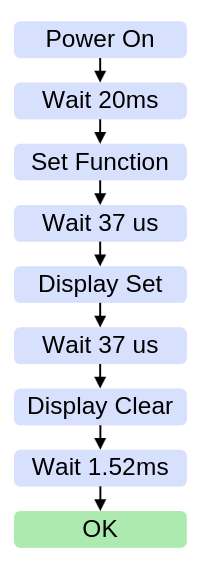
\includegraphics[width=\linewidth]{./images/lcd_timing.png} % replace with your image filename
        \end{minipage}
        \caption{Startup Sequence}
        \label{fig:startup_sequence}
    \end{figure}
    \newline
    Graphik \ref{fig:startup_sequence} zeigt beispielhaft die Initialisierung des Displays und die damit verbundenen Timing-Anforderungen.
    \item \textit{Submodul 2}: LCD Controller  \newline
    Hier werden Befehle interpretiert und die Daten in die entsprechenden Register geschrieben, um die Werte anschließend auf dem Display darzustellen.
    \item \textit{Submodul 3}: AXI Slave Interface  \newline
    Nachdem die Zuverlässigkeit der IP mittels Tests sichergestellt wurde, soll die IP an den internen Systembus (AXI) angebunden werden.
\end{itemize}

Das Registermapping ist an \textit{at\_doc.pdf} aus \textit{02b\_tut\_vhdl\_v03} angelehnt.

\section{Registermapping}

\subsection{I/Os}
\begin{longtable}{|p{4cm}|p{1cm}|p{2cm}|p{6.6cm}|}
\hline
\textbf{Signal Name} & \textbf{I/O} & \textbf{Initial State} & \textbf{Description} \\
\hline
ap\_clk(s00\_axi\_aclk) & I & NA & AXI Clock \\
\hline
ap\_rst\_n (s00\_axi\_aresetn) & I & NA & AXI Reset, active-Low \\
\hline
s\_axi\_control* (s00\_axi*) & NA & NA & AXI4-Lite Slave Interface signals \\
\hline
interrupt & I & 0x0 & Indicates that the condition for an interrupt has occurred. (new sensor value available)
\newline 0 = No interrupt has occurred
\newline 1 = Interrupt has occurred \\
\hline
db4\_7 & O & 0xFF & 4 data bits, necessary in nibble mode. \\
\hline
register\_select & O & 0x1 & Register Select: High for Data Transfer, Low for Instruction Transfer \\
\hline
read\_write & O & 0x1 & Read/Write signal: High for Read mode, Low for Write mode \\
\hline
read\_write\_enable & O & 0x1 & Read/Write Enable: High for Read, falling edge writes data \\
\hline
\caption{PmodCLP Überblick I/O}
\end{longtable}

\subsection{Registerbereich}
% PmodCLP Controller Register Mapping in LaTeX with longtables
% Register Space Overview Table
\begin{longtable}{|p{3cm}|p{3cm}|p{8cm}|}
    \hline
    \textbf{Address Offset} & \textbf{Register Name} & \textbf{Description} \\
    \hline
    \endfirsthead
    \hline
    \textbf{Address Offset} & \textbf{Register Name} & \textbf{Description} \\
    \hline
    \endhead
    \hline \multicolumn{3}{|r|}{{Continued on next page}} \\ \hline
    \endfoot
    \hline
    \endlastfoot

    0x00 & GCSR & General/Global Control and Status Register \\
    \hline
    0x04 & GIER & Global Interrupt Enable Register \\
    \hline
    0x08 & IPIER & IP Interrupt Enable Register \\
    \hline
    0x0C & IPISR & IP Interrupt Status Register \\
    \hline
    0x10 & IDR & ID Register \\
    \hline
    0x14 & VERR & Version Register \\
    \hline
    0x18 & SCSR0 & Special Control and Status Register \\
    \hline
    0x1C & CCR & Character Control Register \\
    \hline
    0x20 & CDR & Character Data Register \\
    \hline
    0x24 & DCR & Display Control Register \\
    \hline
    \caption{PmodCLP Controller Register Space Overview}
    \label{tab:register_overview}
    \end{longtable}

    % GCSR Register Table
    \begin{longtable}{|p{1cm}|p{3cm}|p{2cm}|p{1cm}|p{6.25cm}|}
    \hline
    \textbf{Bit} & \textbf{Name} & \textbf{Access Type} & \textbf{Reset Value} & \textbf{Description} \\
    \hline
    \endfirsthead
    \hline
    \textbf{Bit} & \textbf{Name} & \textbf{Access Type} & \textbf{Reset Value} & \textbf{Description} \\
    \hline
    \endhead
    \hline \multicolumn{5}{|r|}{{Continued on next page}} \\ \hline
    \endfoot
    \hline
    \endlastfoot

    \multicolumn{5}{|c|}{\textbf{0x00 GCSR - General/Global Control and Status Register}} \\
    \hline
    0 & ap\_start & R/W & 0 & Asserted when the kernel can start processing data or format display. Cleared on handshake with ap\_done being asserted. \\
    \hline
    1 & ap\_done & R & 0 & Asserted when the kernel has completed processing data (with or without error). Cleared on read. \\
    \hline
    2 & ap\_idle & R & 0 & Asserted when the kernel is idle. \\
    \hline
    3 & \textit{reserved (ap\_ready)} & R & 0 & Asserted by the kernel when it is ready to accept new data (used only by AP\_CTRL\_CHAIN) \\
    \hline
    4 & \textit{reserved (ap\_continue)} & R/W & 0 & Asserted by the XRT to allow kernel keep running (used only by AP\_CTRL\_CHAIN) \\
    \hline
    5:6 & reserved & & & \\
    \hline
    7 & auto\_restart \textit{(optional)} & R/W & 0 & Used to enable automatic kernel restart. This bit determines whether the display reloads the last sensor value and continues running or clears the display. \\
    \hline
    31:8 & reserved & & & \\
    \hline
    \caption{General/Global Control and Status Register (GCSR)}
    \label{tab:gcsr}
    \end{longtable}

    % GIER Register Table
    \begin{longtable}{|p{1cm}|p{3cm}|p{2cm}|p{1cm}|p{6.25cm}|}
    \hline
    \textbf{Bit} & \textbf{Name} & \textbf{Access Type} & \textbf{Reset Value} & \textbf{Description} \\
    \hline
    \endfirsthead
    \hline
    \textbf{Bit} & \textbf{Name} & \textbf{Access Type} & \textbf{Reset Value} & \textbf{Description} \\
    \hline
    \endhead
    \hline \multicolumn{5}{|r|}{{Continued on next page}} \\ \hline
    \endfoot
    \hline
    \endlastfoot

    \multicolumn{5}{|c|}{\textbf{0x04 GIER - Global Interrupt Enable Register}} \\
    \hline
    0 & gie & R/W & 0 & When asserted, along with the IP Interrupt Enable bit, the interrupt is enabled. \\
    \hline
    31:1 & reserved & & & \\
    \hline
    \caption{Global Interrupt Enable Register (GIER)}
    \label{tab:gier}
    \end{longtable}

    % IPIER Register Table
    \begin{longtable}{|p{1cm}|p{3cm}|p{2cm}|p{1cm}|p{6.25cm}|}
    \hline
    \textbf{Bit} & \textbf{Name} & \textbf{Access Type} & \textbf{Reset Value} & \textbf{Description} \\
    \hline
    \endfirsthead
    \hline
    \textbf{Bit} & \textbf{Name} & \textbf{Access Type} & \textbf{Reset Value} & \textbf{Description} \\
    \hline
    \endhead
    \hline \multicolumn{5}{|r|}{{Continued on next page}} \\ \hline
    \endfoot
    \hline
    \endlastfoot

    \multicolumn{5}{|c|}{\textbf{0x08 IPIER - IP Interrupt Enable Register}} \\
    \hline
    0 & ipie & R/W & 0 & When asserted, along with Global Interrupt Enable bit, the interrupt is enabled. (default: uses the internal ap\_done signal to trigger an interrupt) \\
    \hline
    31:1 & reserved & & & \\
    \hline
    \caption{IP Interrupt Enable Register (IPIER)}
    \label{tab:ipier}
    \end{longtable}

    % IPISR Register Table
    \begin{longtable}{|p{1cm}|p{3cm}|p{2cm}|p{1cm}|p{6.25cm}|}
    \hline
    \textbf{Bit} & \textbf{Name} & \textbf{Access Type} & \textbf{Reset Value} & \textbf{Description} \\
    \hline
    \endfirsthead
    \hline
    \textbf{Bit} & \textbf{Name} & \textbf{Access Type} & \textbf{Reset Value} & \textbf{Description} \\
    \hline
    \endhead
    \hline \multicolumn{5}{|r|}{{Continued on next page}} \\ \hline
    \endfoot
    \hline
    \endlastfoot

    \multicolumn{5}{|c|}{\textbf{0x0C IPISR - IP Interrupt Status Register}} \\
    \hline
    0 & ipis & R/W & 0 & Toggle on write. (write 1 to clear(W1C)) \\
    \hline
    31:1 & reserved & & & \\
    \hline
    \caption{IP Interrupt Status Register (IPISR)}
    \label{tab:ipisr}
    \end{longtable}

    % IDR Register Table
    \begin{longtable}{|p{1cm}|p{3cm}|p{2cm}|p{2.5cm}|p{4.75cm}|}
    \hline
    \textbf{Bit} & \textbf{Name} & \textbf{Access Type} & \textbf{Reset Value} & \textbf{Description} \\
    \hline
    \endfirsthead
    \hline
    \textbf{Bit} & \textbf{Name} & \textbf{Access Type} & \textbf{Reset Value} & \textbf{Description} \\
    \hline
    \endhead
    \hline \multicolumn{5}{|r|}{{Continued on next page}} \\ \hline
    \endfoot
    \hline
    \endlastfoot

    \multicolumn{5}{|c|}{\textbf{0x10 IDR - ID Register}} \\
    \hline
    31:0 & ID & R & 0x80010744 & Distinct ID for PmodCLP Controller \\
    \hline
    \caption{ID Register (IDR)}
    \label{tab:idr}
    \end{longtable}

    % VERR Register Table
    \begin{longtable}{|p{1cm}|p{3cm}|p{2cm}|p{2.5cm}|p{4.75cm}|}
    \hline
    \textbf{Bit} & \textbf{Name} & \textbf{Access Type} & \textbf{Reset Value} & \textbf{Description} \\
    \hline
    \endfirsthead
    \hline
    \textbf{Bit} & \textbf{Name} & \textbf{Access Type} & \textbf{Reset Value} & \textbf{Description} \\
    \hline
    \endhead
    \hline \multicolumn{5}{|r|}{{Continued on next page}} \\ \hline
    \endfoot
    \hline
    \endlastfoot

    \multicolumn{5}{|c|}{\textbf{0x14 VERR - Version Register}} \\
    \hline
    31:0 & VER & R & 0x80001000 & Version \\
    \hline
    \caption{Version Register (VERR)}
    \label{tab:verr}
    \end{longtable}

    % SCSR0 Register Table
    \begin{longtable}{|p{1cm}|p{3cm}|p{2cm}|p{1cm}|p{6.25cm}|}
    \hline
    \textbf{Bit} & \textbf{Name} & \textbf{Access Type} & \textbf{Reset Value} & \textbf{Description} \\
    \hline
    \endfirsthead
    \hline
    \textbf{Bit} & \textbf{Name} & \textbf{Access Type} & \textbf{Reset Value} & \textbf{Description} \\
    \hline
    \endhead
    \hline \multicolumn{5}{|r|}{{Continued on next page}} \\ \hline
    \endfoot
    \hline
    \endlastfoot

    \multicolumn{5}{|c|}{\textbf{0x18 SCSR0 - Special Control and Status Register}} \\
    \hline
    0 & lcd\_initialized & R & 0 & 1 indicates the LCD has been properly initialized and is ready for commands. \\
    \hline
    8:1 & lcd\_state \textit{(for debugging)} & R & 0x00 & Current state of LCD controller. (startup: 0x00, init: 0x01, ready: 0x02, write: 0x04, read: 0x08, clear display: 0x10, return home: 0x14, display control: 0x18, display line switch: 0x1C) \\
    \hline
    9 & lcd\_error\_flag & R & 0 & Indicates an error occurred during last operation. In combination with 'write\_char' and 'read\_char' two errors can occur: invalid symbol (write) or invalid ddram pos (read). \\
    \hline
    31:10 & reserved & & & \\
    \hline
    \caption{Special Control and Status Register (SCSR0)}
    \label{tab:scsr0}
    \end{longtable}

    % CCR Register Table
    \begin{longtable}{|p{1cm}|p{4cm}|p{1cm}|p{1cm}|p{6.25cm}|}
    \hline
    \textbf{Bit} & \textbf{Name} & \textbf{Access Type} & \textbf{Reset Value} & \textbf{Description} \\
    \hline
    \endfirsthead
    \hline
    \textbf{Bit} & \textbf{Name} & \textbf{Access Type} & \textbf{Reset Value} & \textbf{Description} \\
    \hline
    \endhead
    \hline \multicolumn{5}{|r|}{{Continued on next page}} \\ \hline
    \endfoot
    \hline
    \endlastfoot

    \multicolumn{5}{|c|}{\textbf{0x1C CCR - Character Control Register}} \\
    \hline
    7:0 & ddram\_pos\_last\_written & R & 0xFF & Last updated DDRAM address/position for character (00H-27H for line 1, 40H-67H for line 2)  \\
    \hline
    15:8 & ddram\_pos\_to\_read \textit{(optional)} & R/W & 0xFF & DDRAM address/position for character (00H-27H for line 1, 40H-67H for line 2) for software testing purpose (e.g. read symbol which was written before). \\
    \hline
    16 & write\_char & R/W & 0 & Write 1 to initiate character write either to specified DDRAM position (if ddram\_pos is in valid range) or default last\_ddram\_pos. \\
    \hline
    17 & read\_char \textit{(optional)} & R/W & 0 & Write 1 to read character either from specified DDRAM position (if ddram\_pos is in valid range) or default last\_ddram\_pos. \\
    \hline
    31:18 & reserved & & & \\
    \hline
    \caption{Character Control Register (CCR)}
    \label{tab:cdr}
    \end{longtable}

    % CDR Register Table
    \begin{longtable}{|p{1cm}|p{3cm}|p{2cm}|p{1cm}|p{6.25cm}|}
    \hline
    \textbf{Bit} & \textbf{Name} & \textbf{Access Type} & \textbf{Reset Value} & \textbf{Description} \\
    \hline
    \endfirsthead
    \hline
    \textbf{Bit} & \textbf{Name} & \textbf{Access Type} & \textbf{Reset Value} & \textbf{Description} \\
    \hline
    \endhead
    \hline \multicolumn{5}{|r|}{{Continued on next page}} \\ \hline
    \endfoot
    \hline
    \endlastfoot
    \multicolumn{5}{|c|}{\textbf{0x20 CDR - Character Data Register}} \\
    \hline
    7:0 & symbol\_to\_write & R/W & 0xFF & Character symbol to write to LCD. \\
    \hline
    15:8 & symbol\_read \textit{(optional)} & R & 0x3F & Character symbol which was read ('?' is default value if no read operation was triggered before). For software testing purpose. \\
    \hline
    31:16 & reserved & & & \\
    \hline
    \caption{Character Data Register (CDR)}
    \label{tab:cdr}
    \end{longtable}

    % DCR Register Table
    \begin{longtable}{|p{1cm}|p{3cm}|p{2cm}|p{1cm}|p{6.25cm}|}
        \hline
        \textbf{Bit} & \textbf{Name} & \textbf{Access Type} & \textbf{Reset Value} & \textbf{Description} \\
        \hline
        \endfirsthead
        \hline
        \textbf{Bit} & \textbf{Name} & \textbf{Access Type} & \textbf{Reset Value} & \textbf{Description} \\
        \hline
        \endhead
        \hline \multicolumn{5}{|r|}{{Continued on next page}} \\ \hline
        \endfoot
        \hline
        \endlastfoot

        \multicolumn{5}{|c|}{\textbf{0x24 DCR - Display Control Register}} \\
        \hline
        0 & clear\_display & R/W & 0 & Write 1 to clear the display \\
        \hline
        1 & return\_home & R/W & 0 & Write 1 to return cursor to home position \\
        \hline
        2 & cursor\_on & R/W & 1 & Enable cursor visibility (0 = off, 1 = on) \\
        \hline
        3 & cursor\_blink & R/W & 1 & Enable cursor blinking (0 = no blink, 1 = blink) \\
        \hline
        4 & cursor\_apply & R/W & 0 & Write 1 to apply cursor formatting set in cursor\_on and cursor\_blink. \\
        \hline
        5 & display\_line \textit{(optional)} & R/W & 0 & Indicates selected line on display (0 = line 1, 1 = line 2) \\
        \hline
        31:6 & reserved & & & \\
        \hline
        \caption{Display Control Register (DCR)}
        \label{tab:fmr}
        \end{longtable}
